\chapter{Anhang A}
\label{chap:anhang_a}

\begin{figure}[ht]
    \centering
    \begin{minipage}[t]{0.45\linewidth}
        \centering
        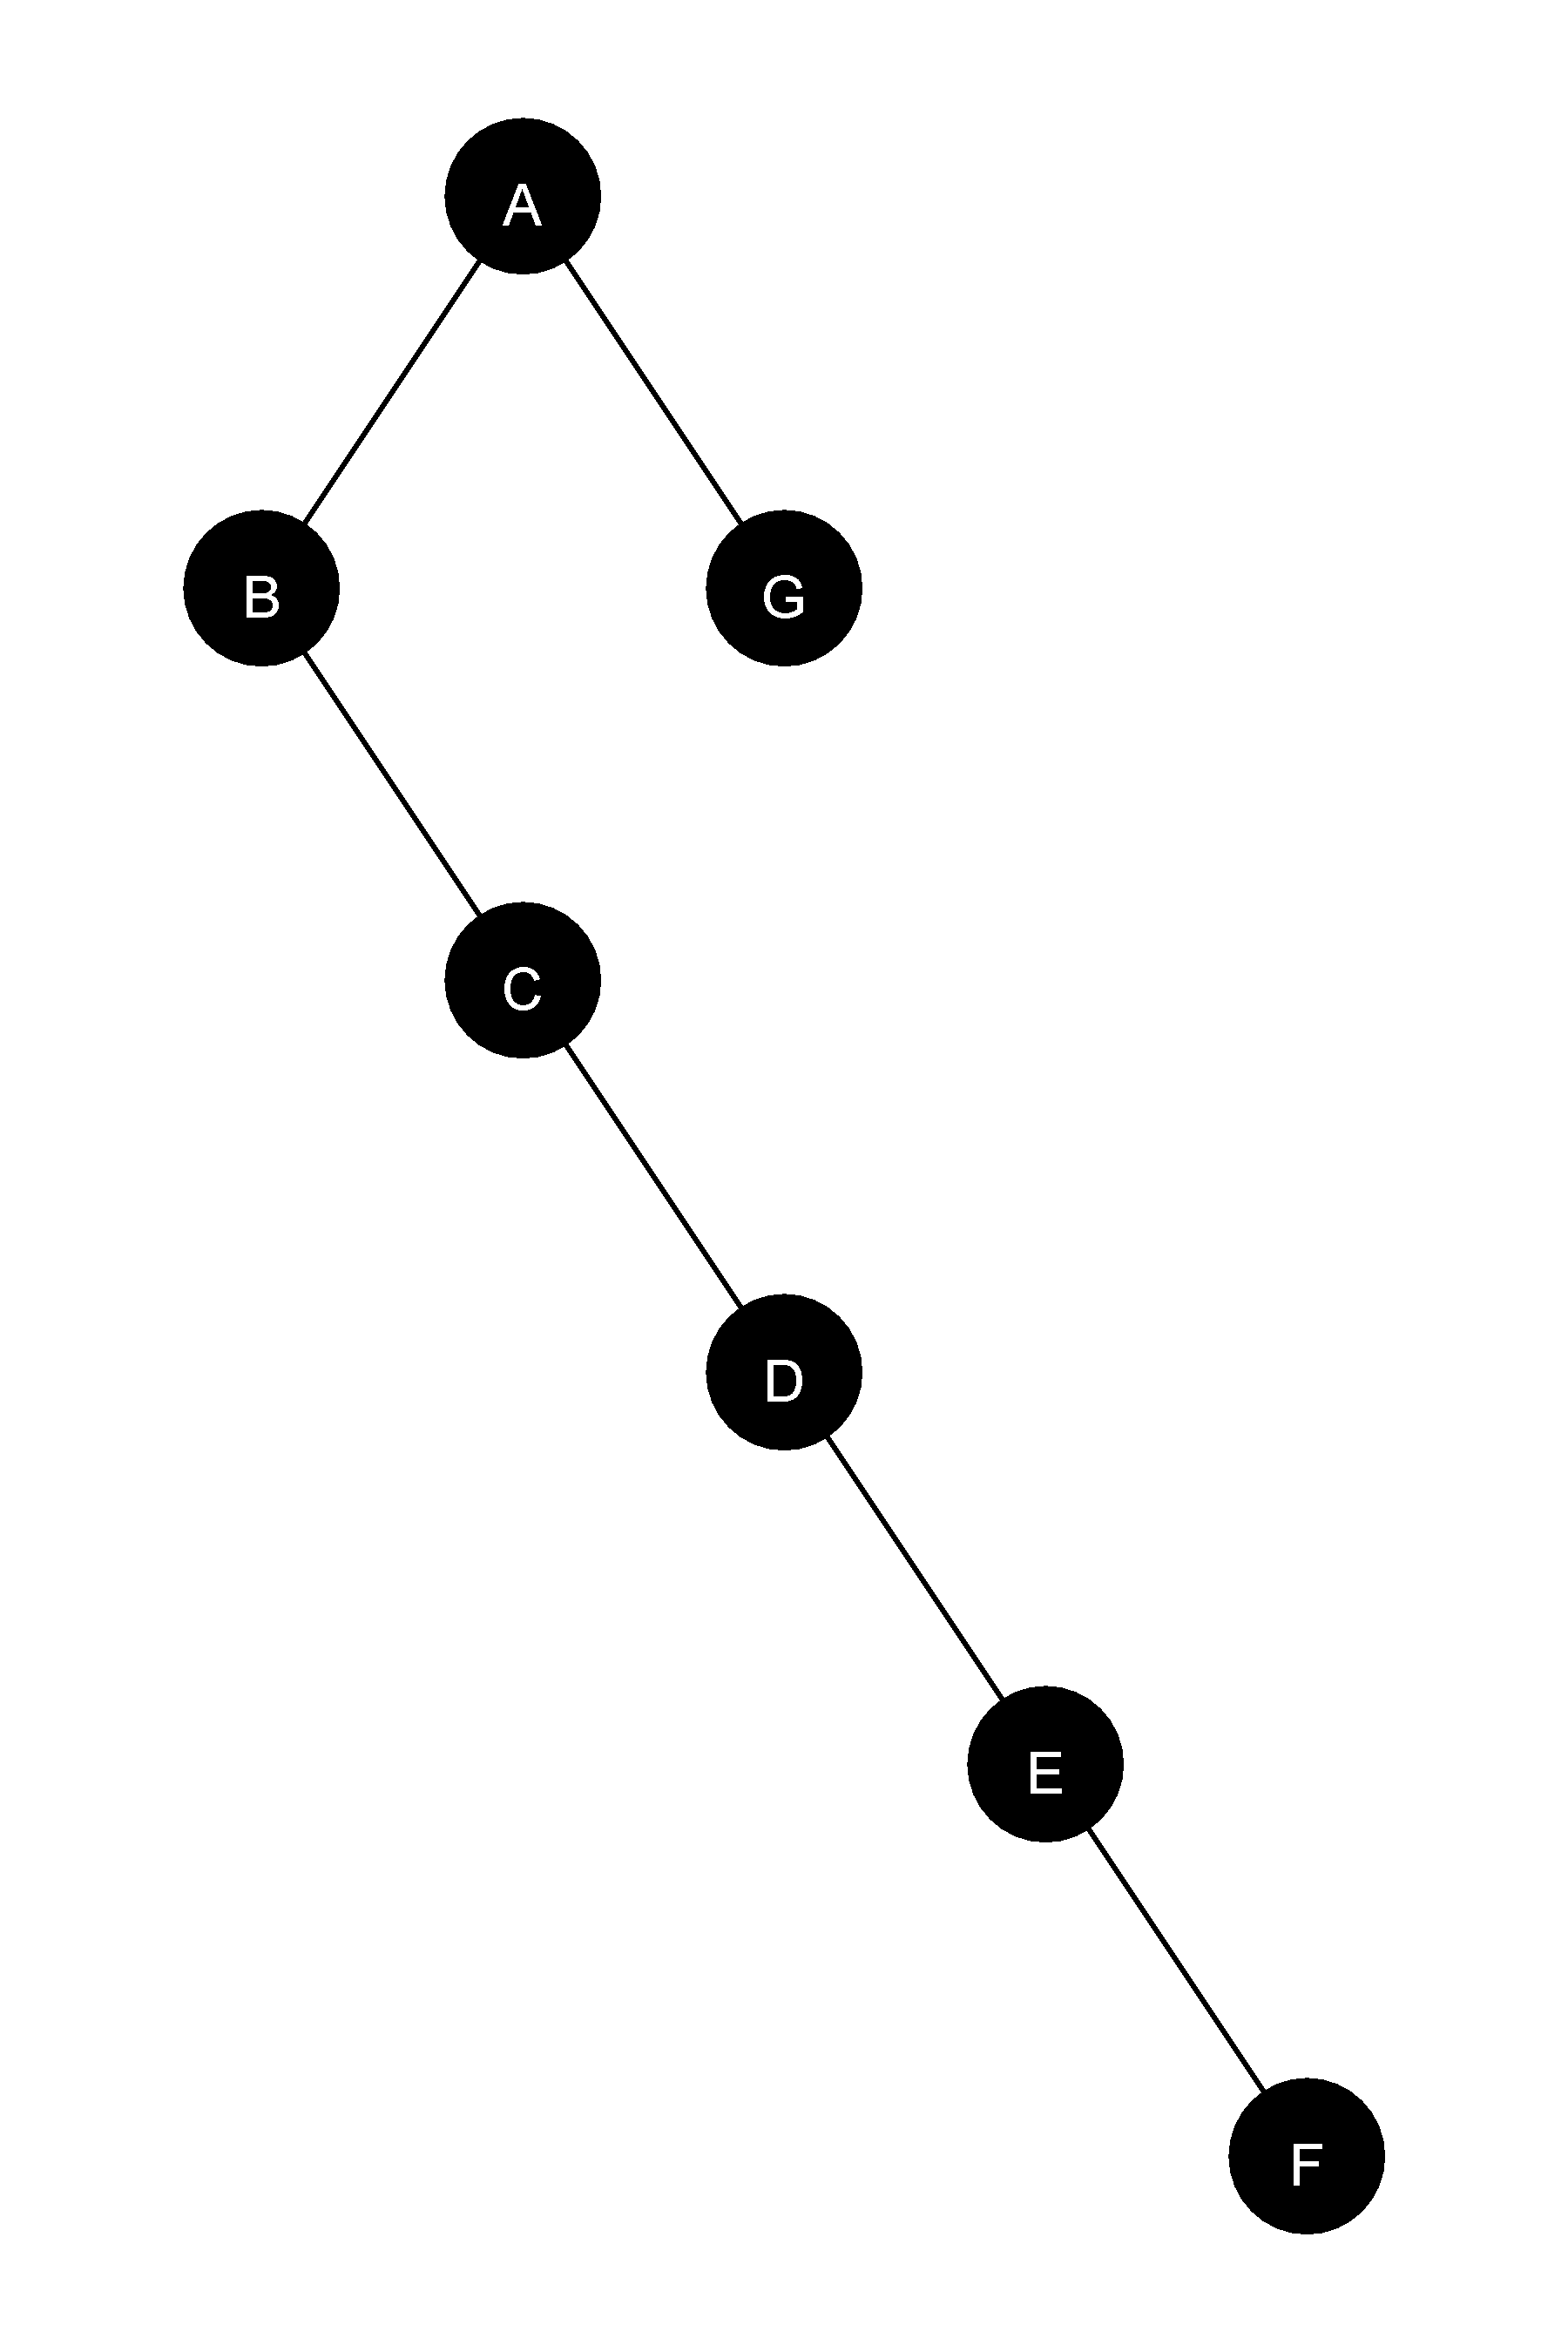
\includegraphics[scale = 0.06]{abbildungen/tree_spiegel_1_a2}
    \end{minipage}
    \hfill
    \begin{minipage}[t]{0.45\linewidth}
        \centering
        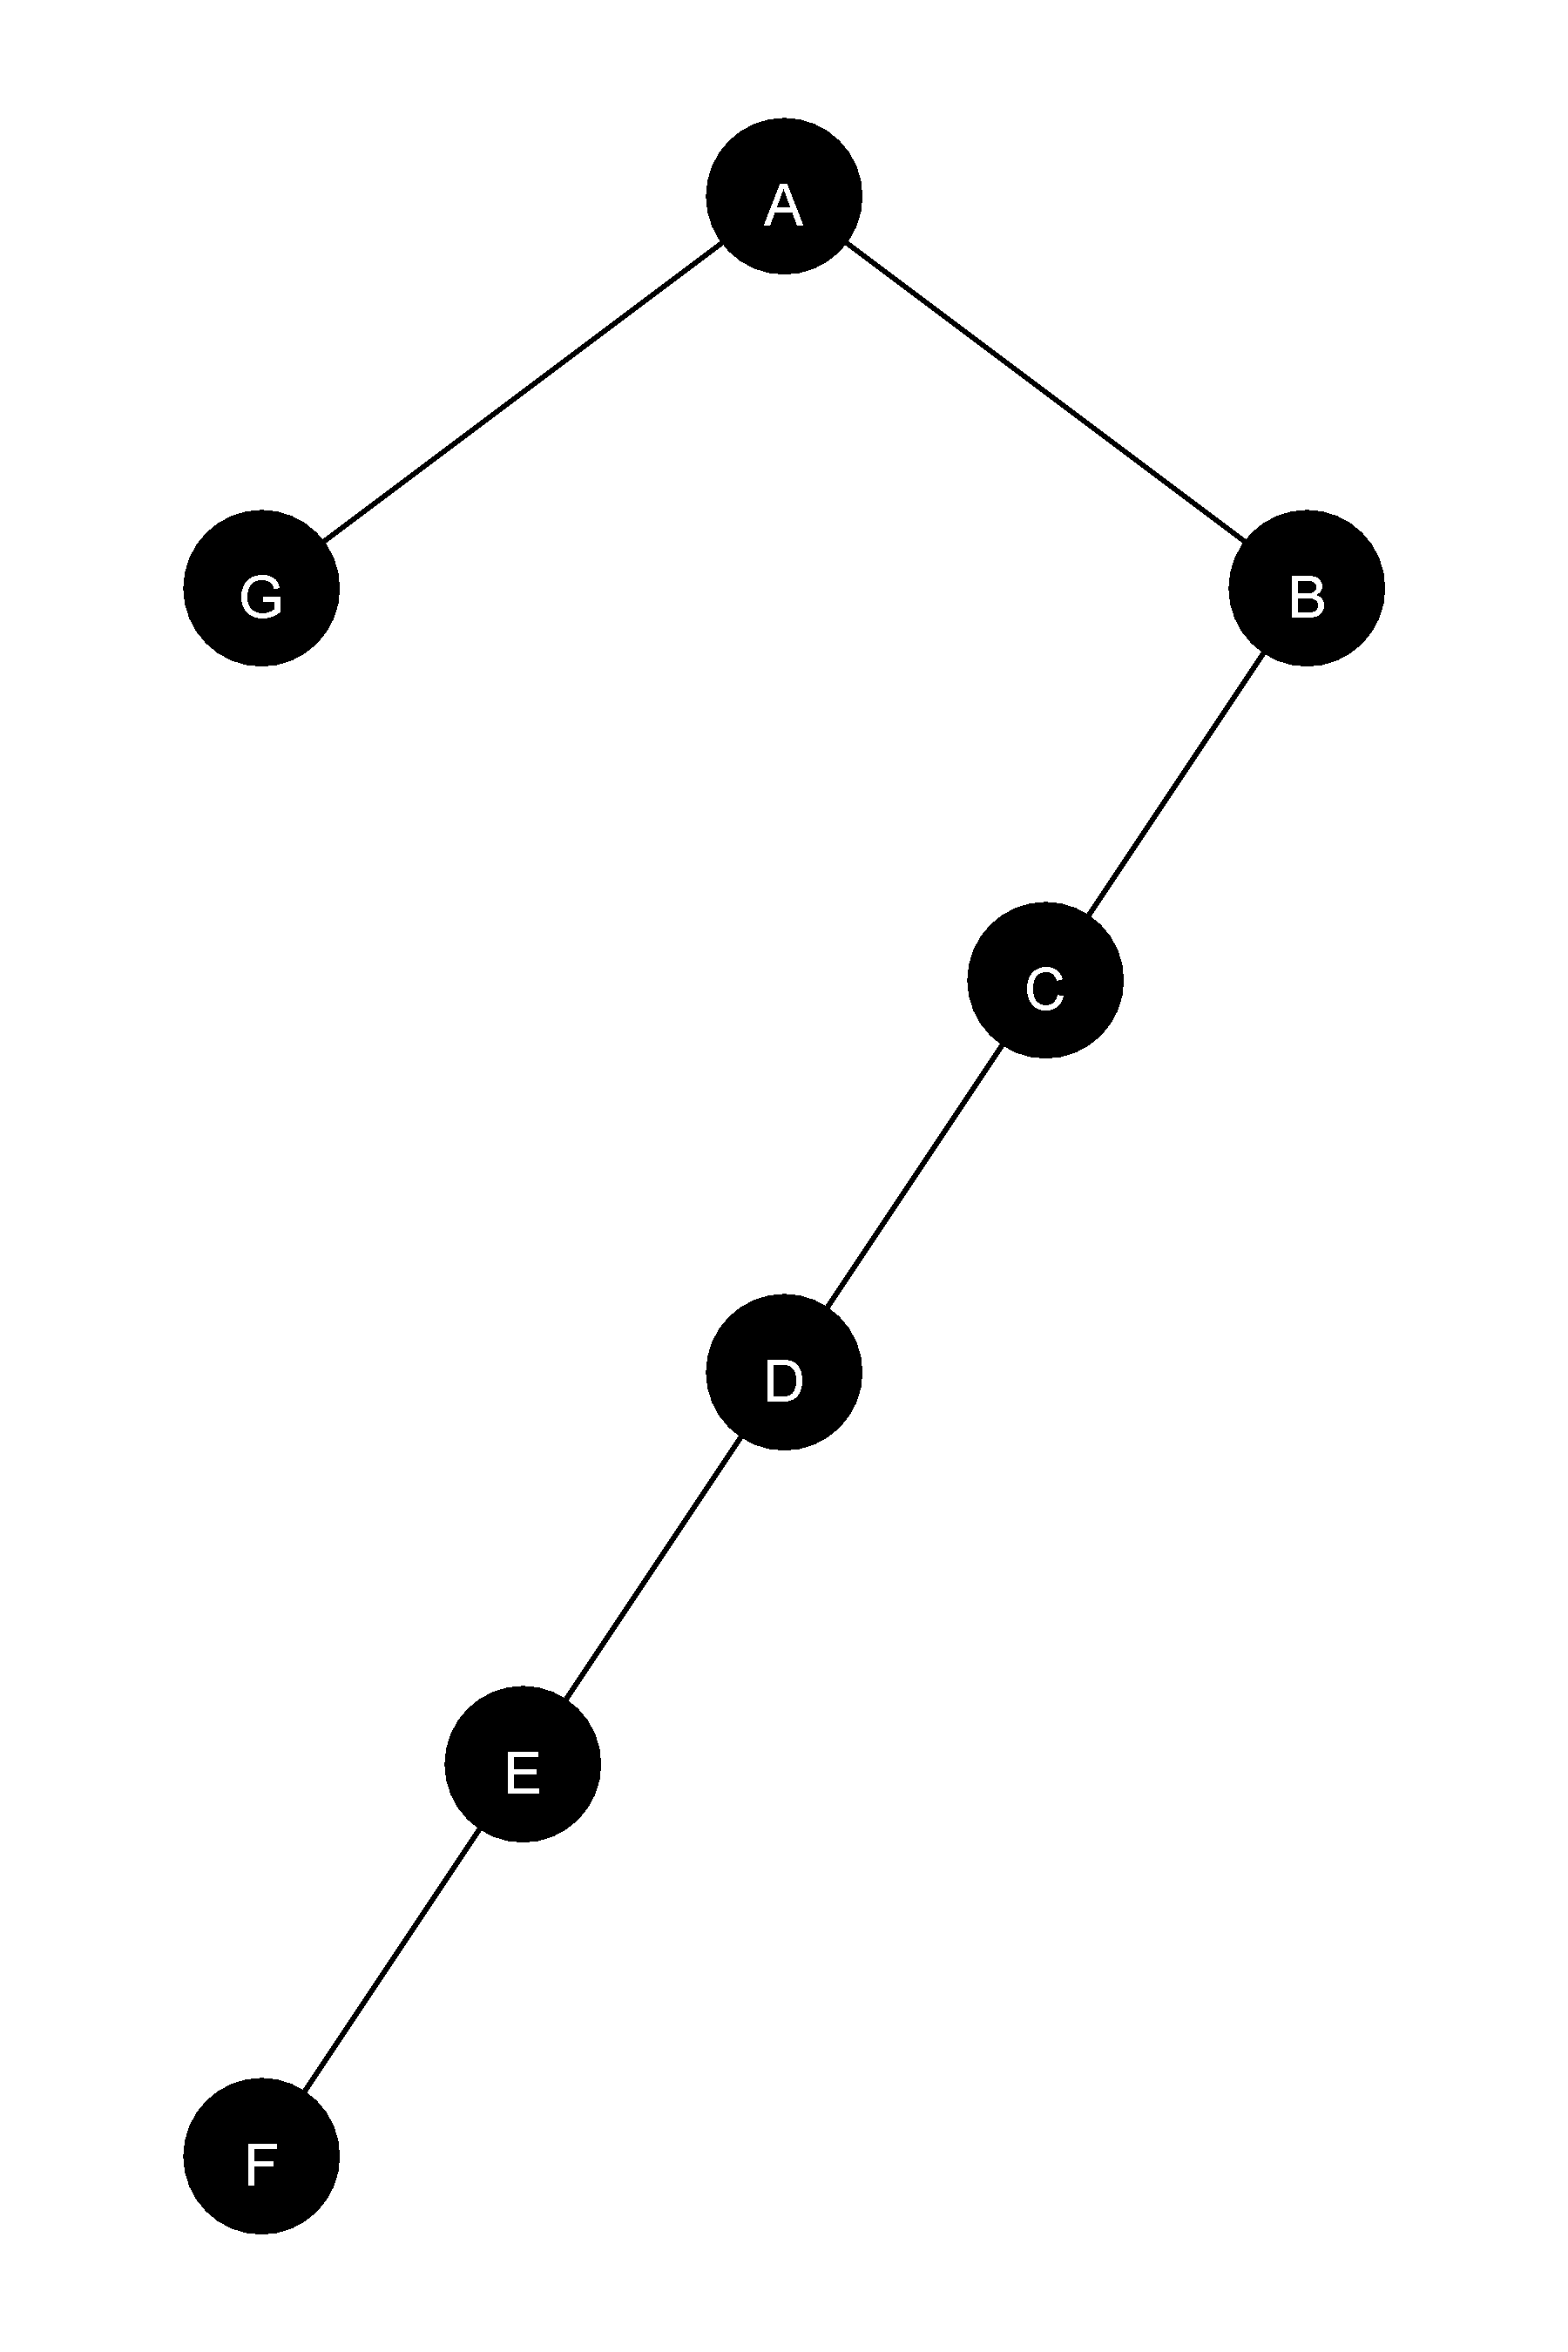
\includegraphics[scale = 0.06]{abbildungen/tree_spiegel_2_a2}
    \end{minipage} 
    \caption[]{Baum und Spiegelung gezeichnet nach WS}
    \label{pic:WS_Spiegel}
\end{figure}

\begin{figure}[ht]
    \centering
    \begin{minipage}[t]{0.45\linewidth}
        \centering
        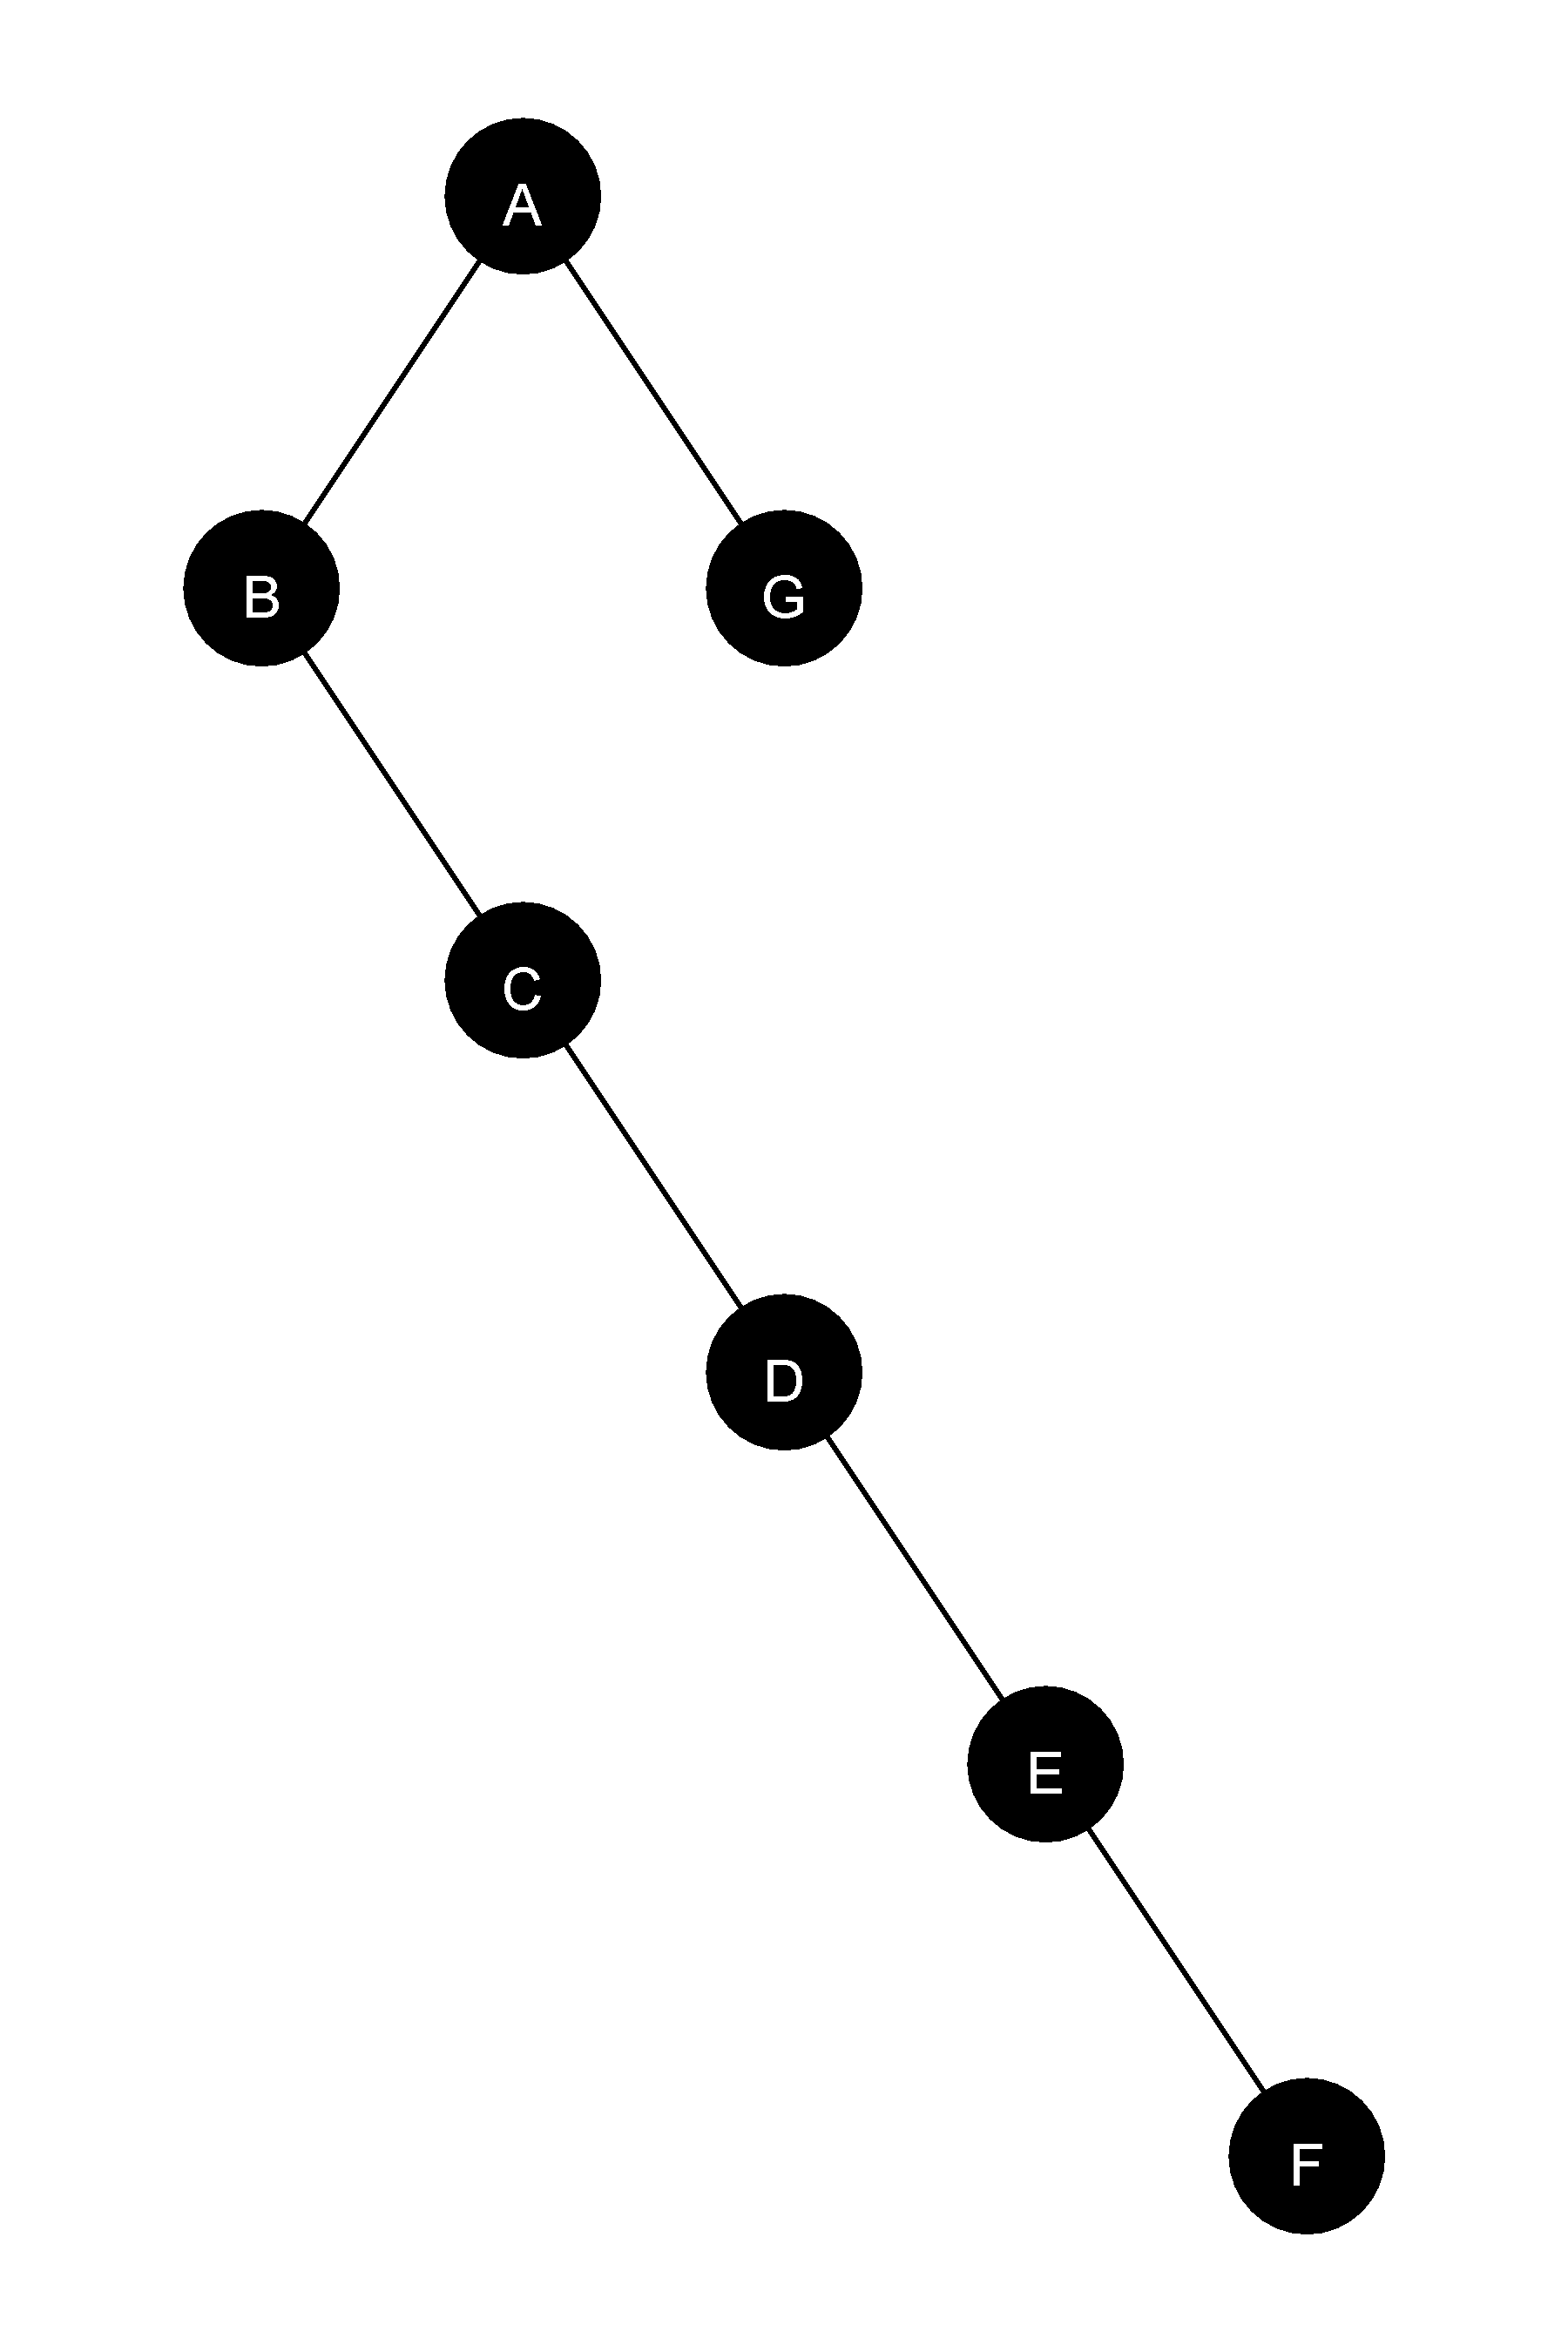
\includegraphics[scale = 0.06]{abbildungen/tree_spiegel_1_a3}
    \end{minipage}
    \hfill
    \begin{minipage}[t]{0.45\linewidth}
        \centering
        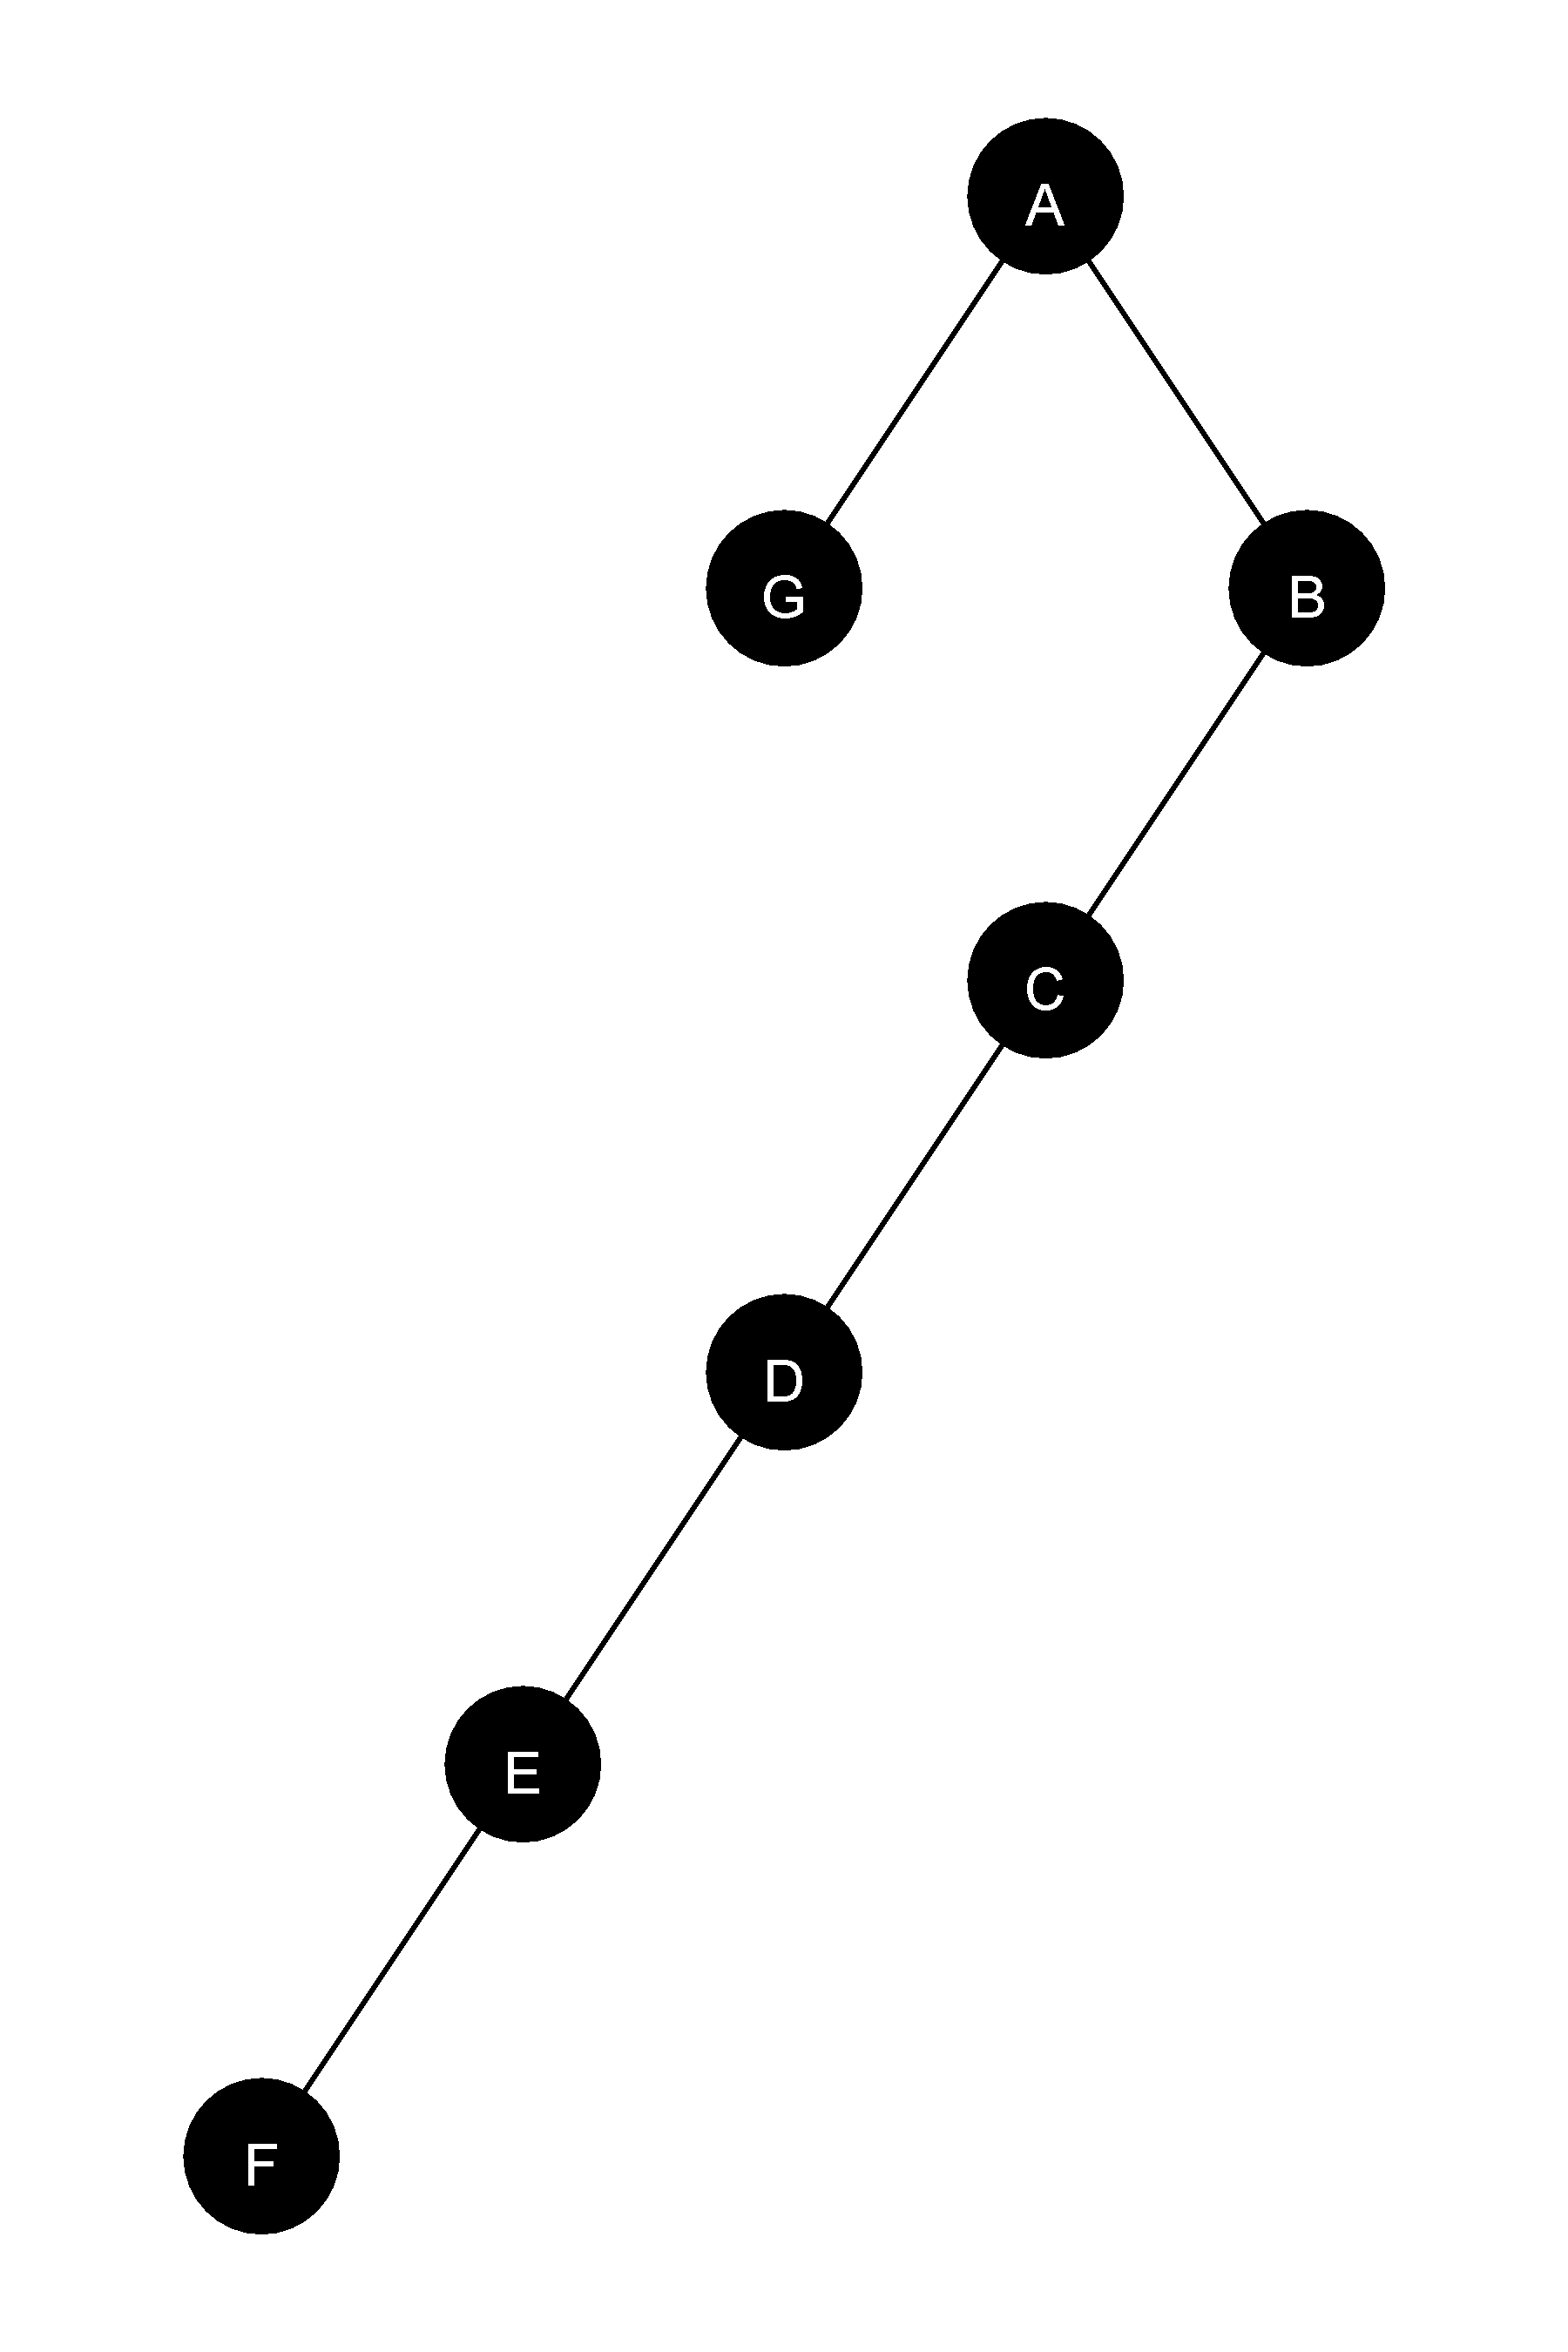
\includegraphics[scale = 0.06]{abbildungen/tree_spiegel_2_a3}   
    \end{minipage}  
    \caption[]{Baum und Spiegelung gezeichnet nach TR}
    \label{pic:TR_Spiegel}
\end{figure}

\begin{figure}[ht]
    \centering
    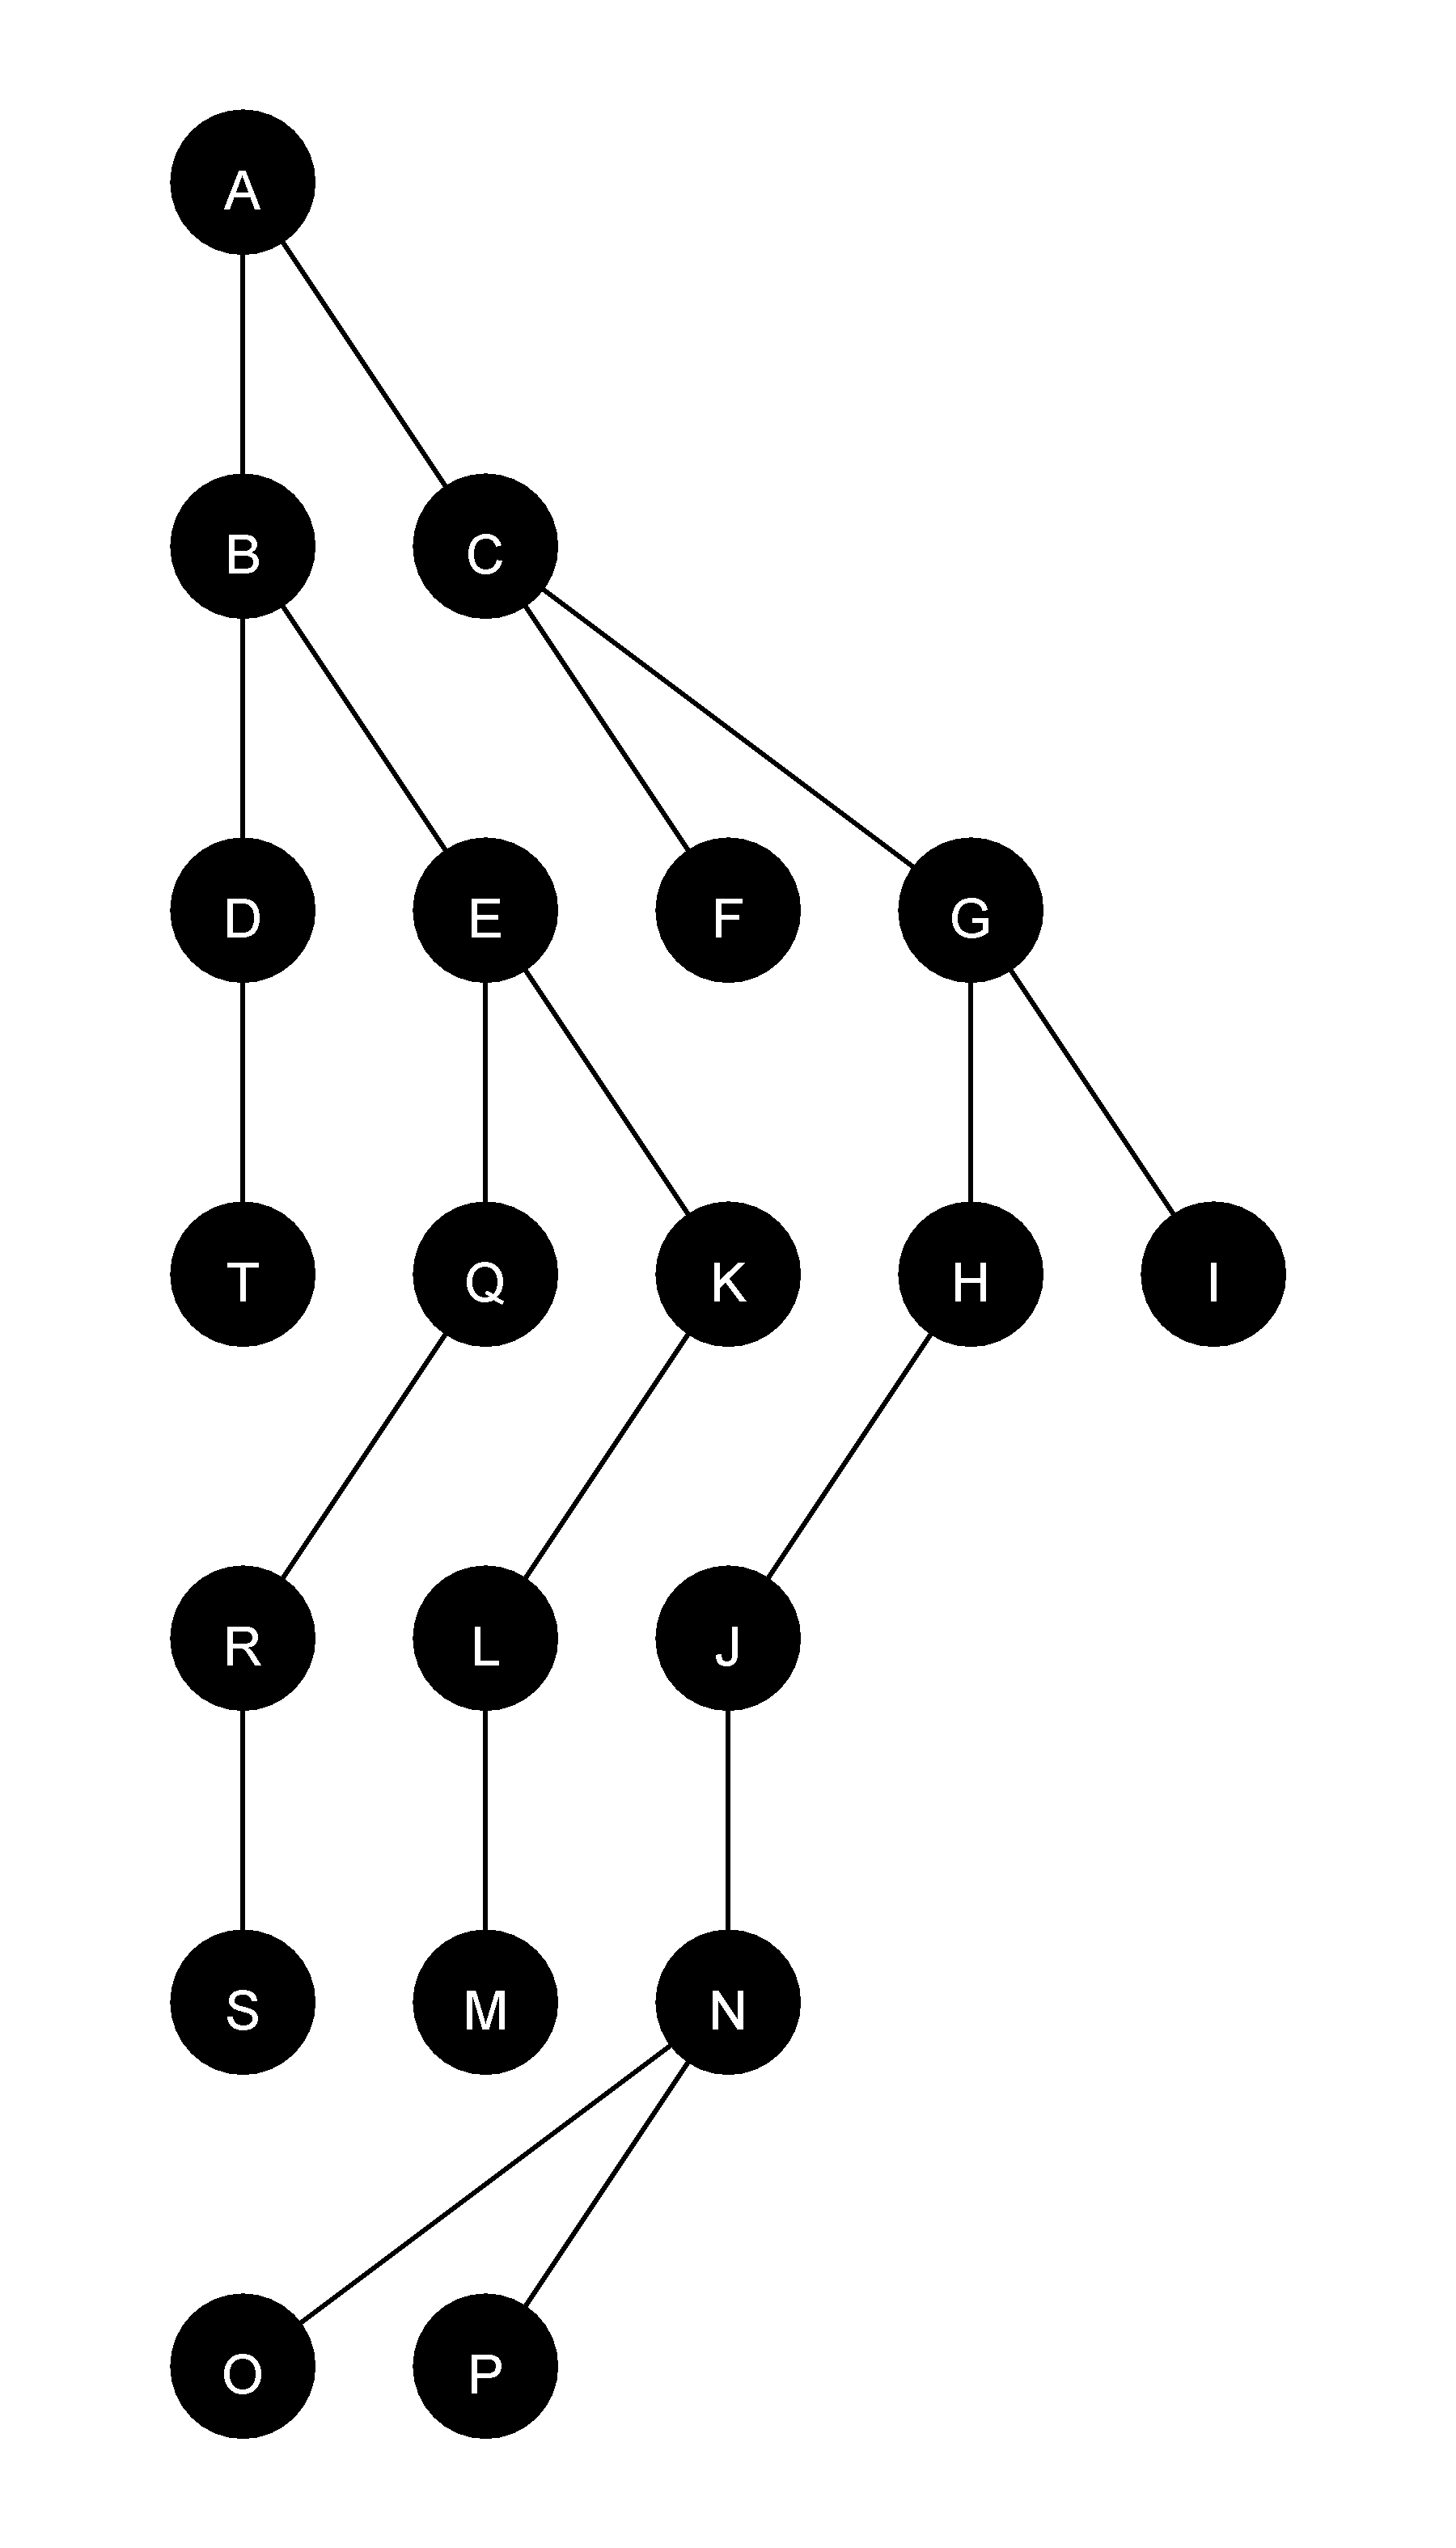
\includegraphics[scale = 0.18]{abbildungen/komplex_a1}
    \caption{Komplexer Baum gezeichnet von naiven WS}
\end{figure}

\begin{figure}[ht]
    \centering
    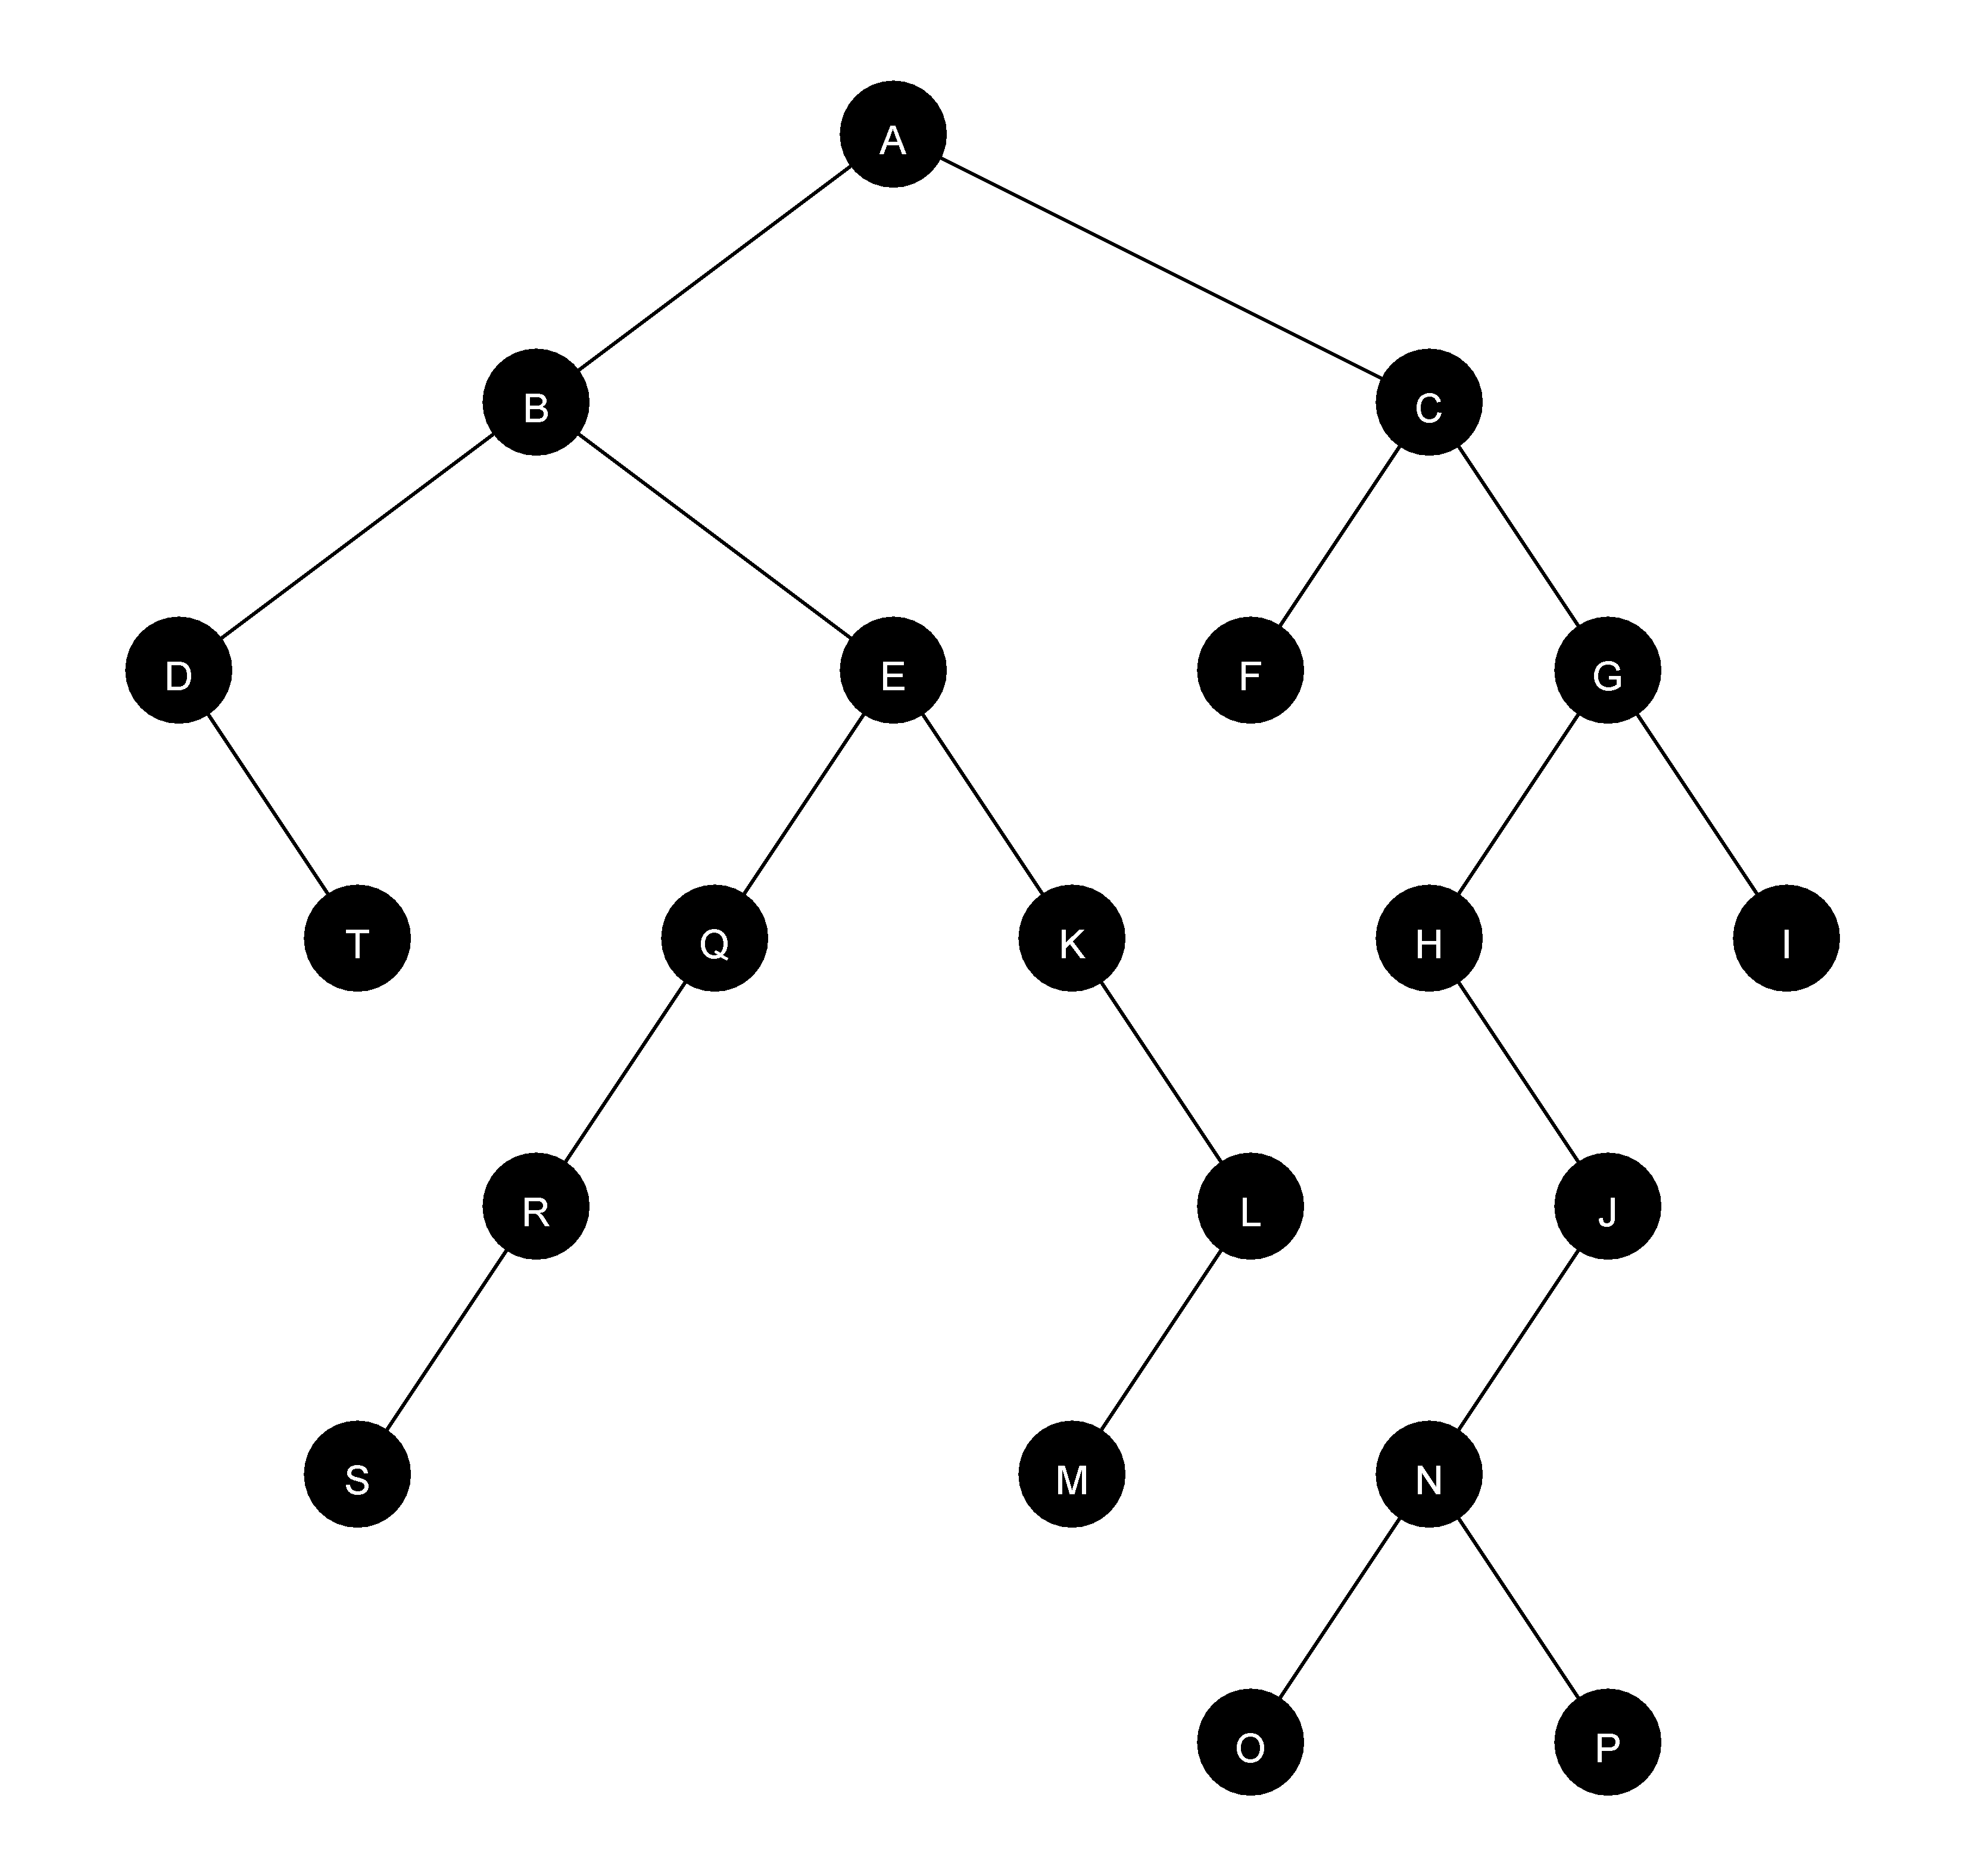
\includegraphics[scale = 0.12]{abbildungen/komplex_a2}
    \caption{Komplexer Baum gezeichnet von WS}
\end{figure}

\begin{figure}[ht]
    \centering
    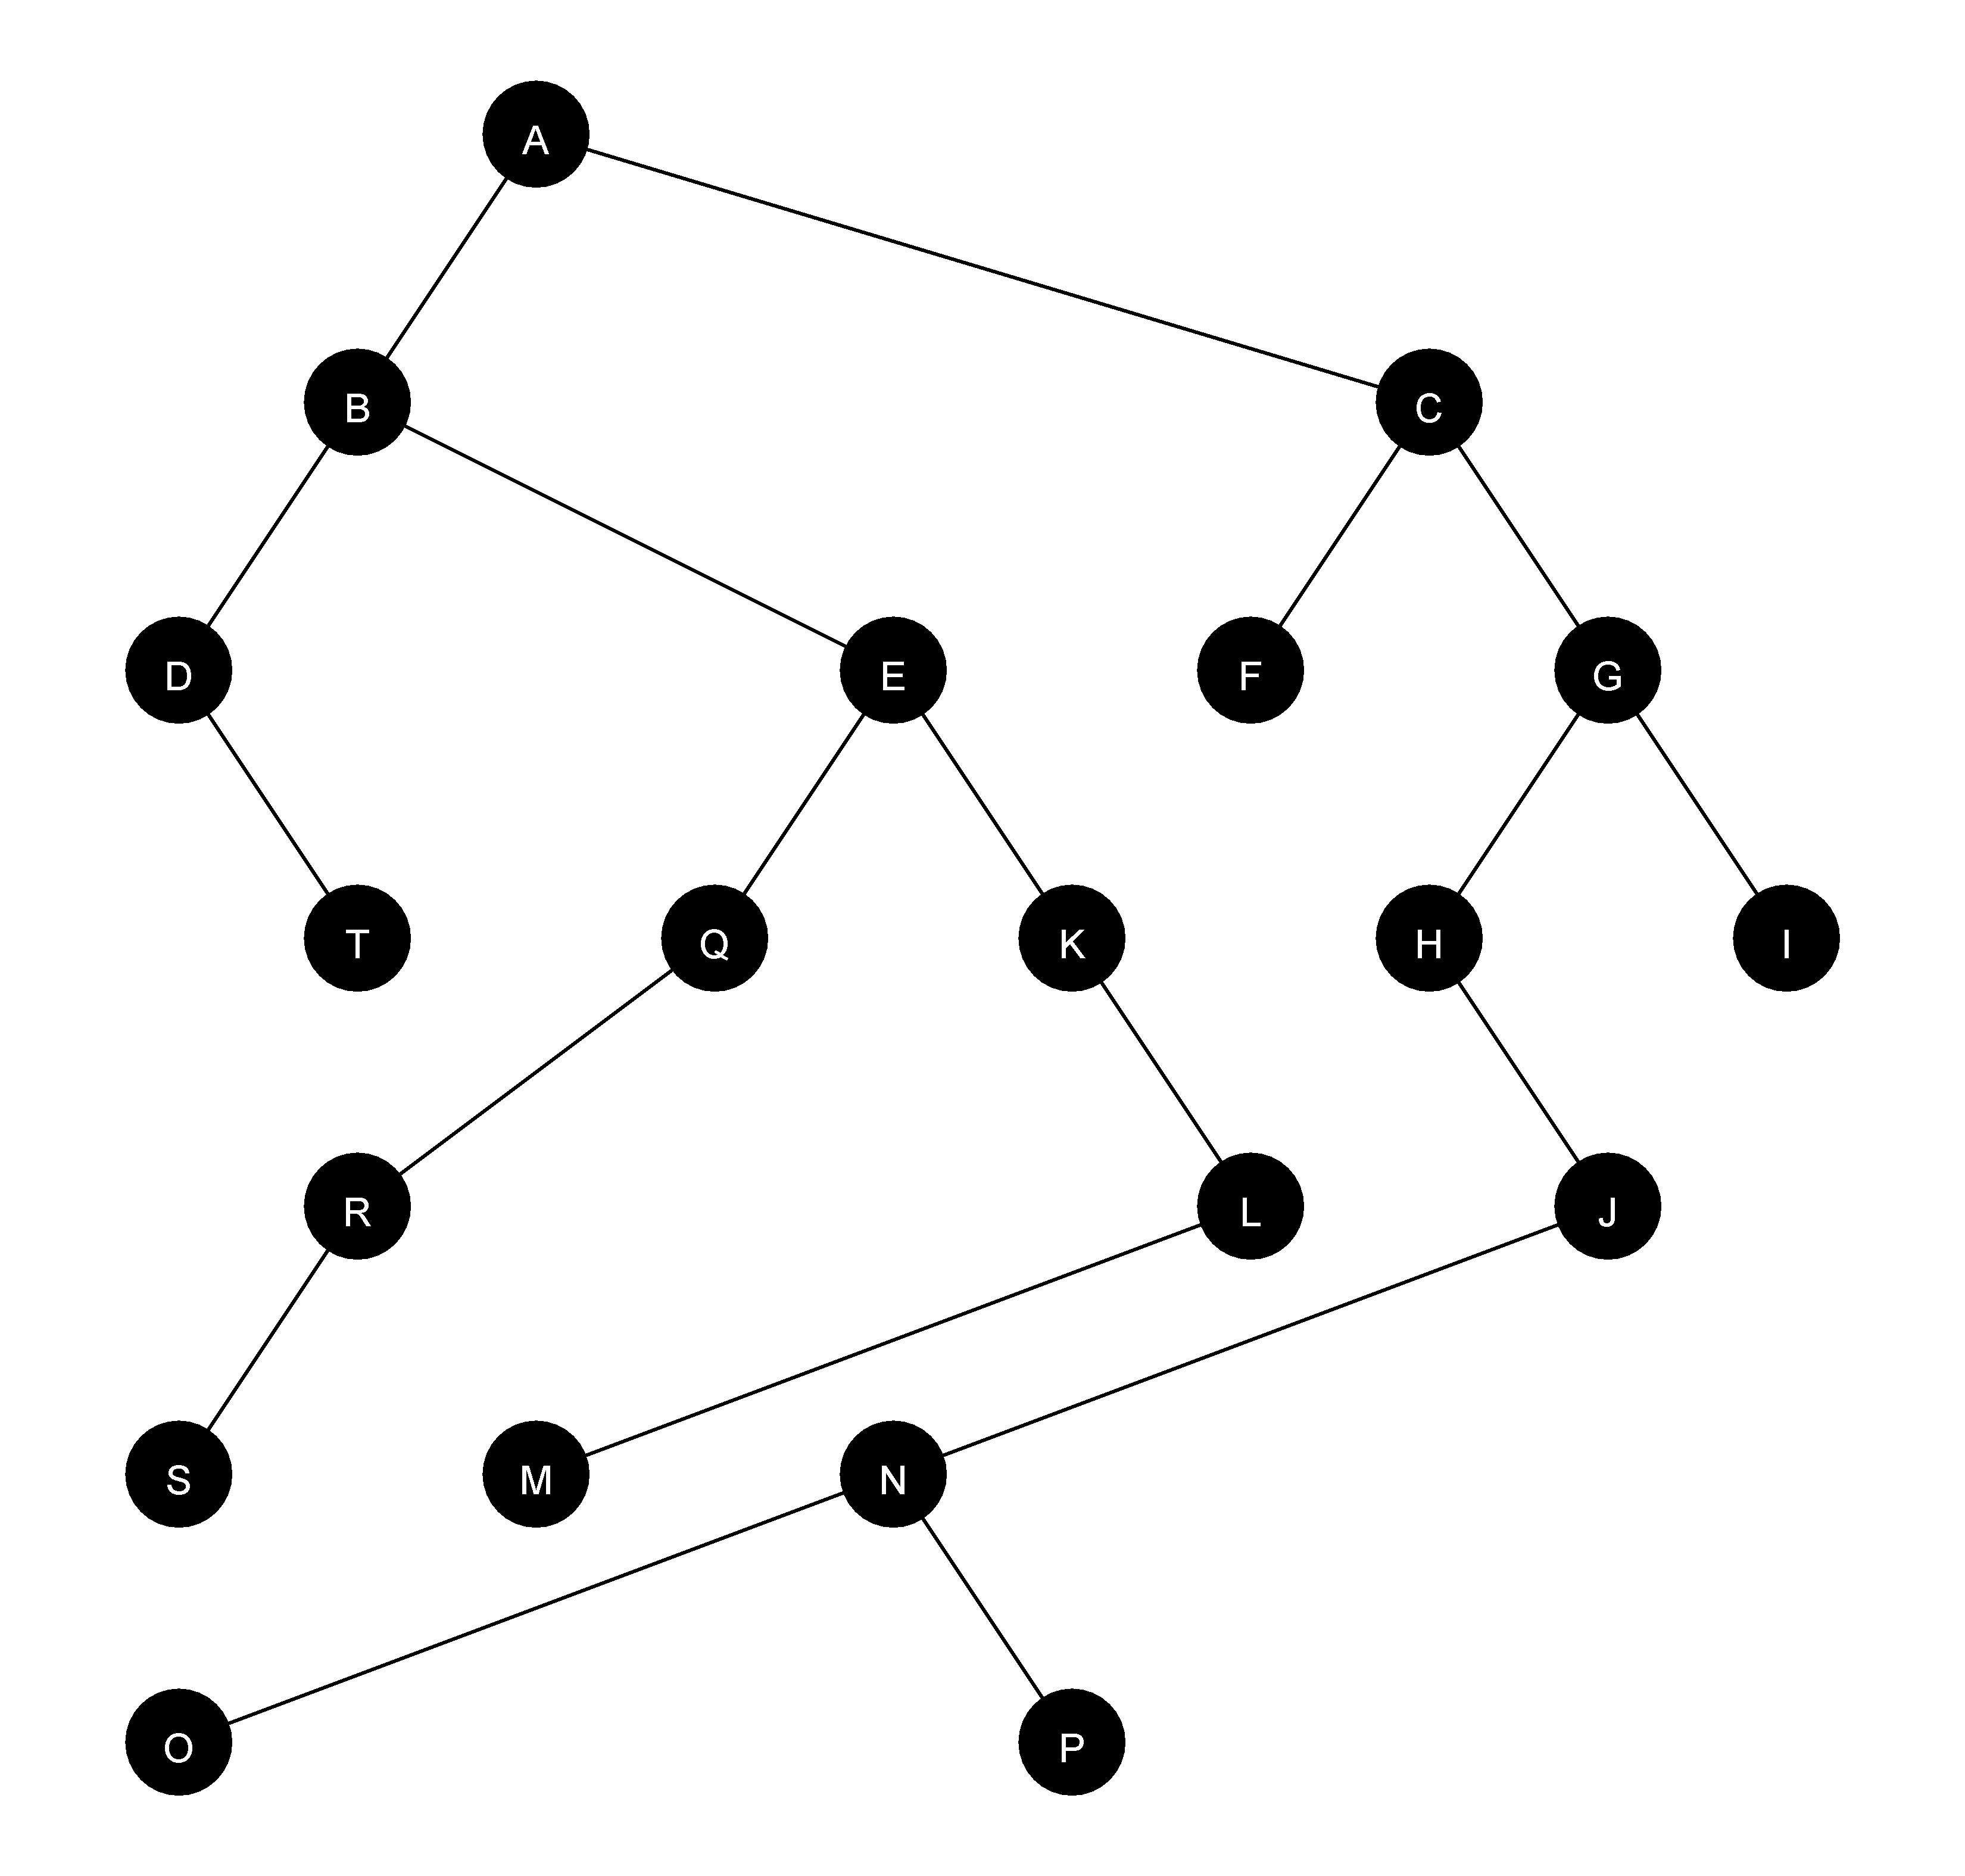
\includegraphics[scale = 0.12]{abbildungen/komplex_a2_v}
    \caption{Komplexer Baum gezeichnet von verbessertem WS}
\end{figure}

\begin{figure}[ht]
    \centering
    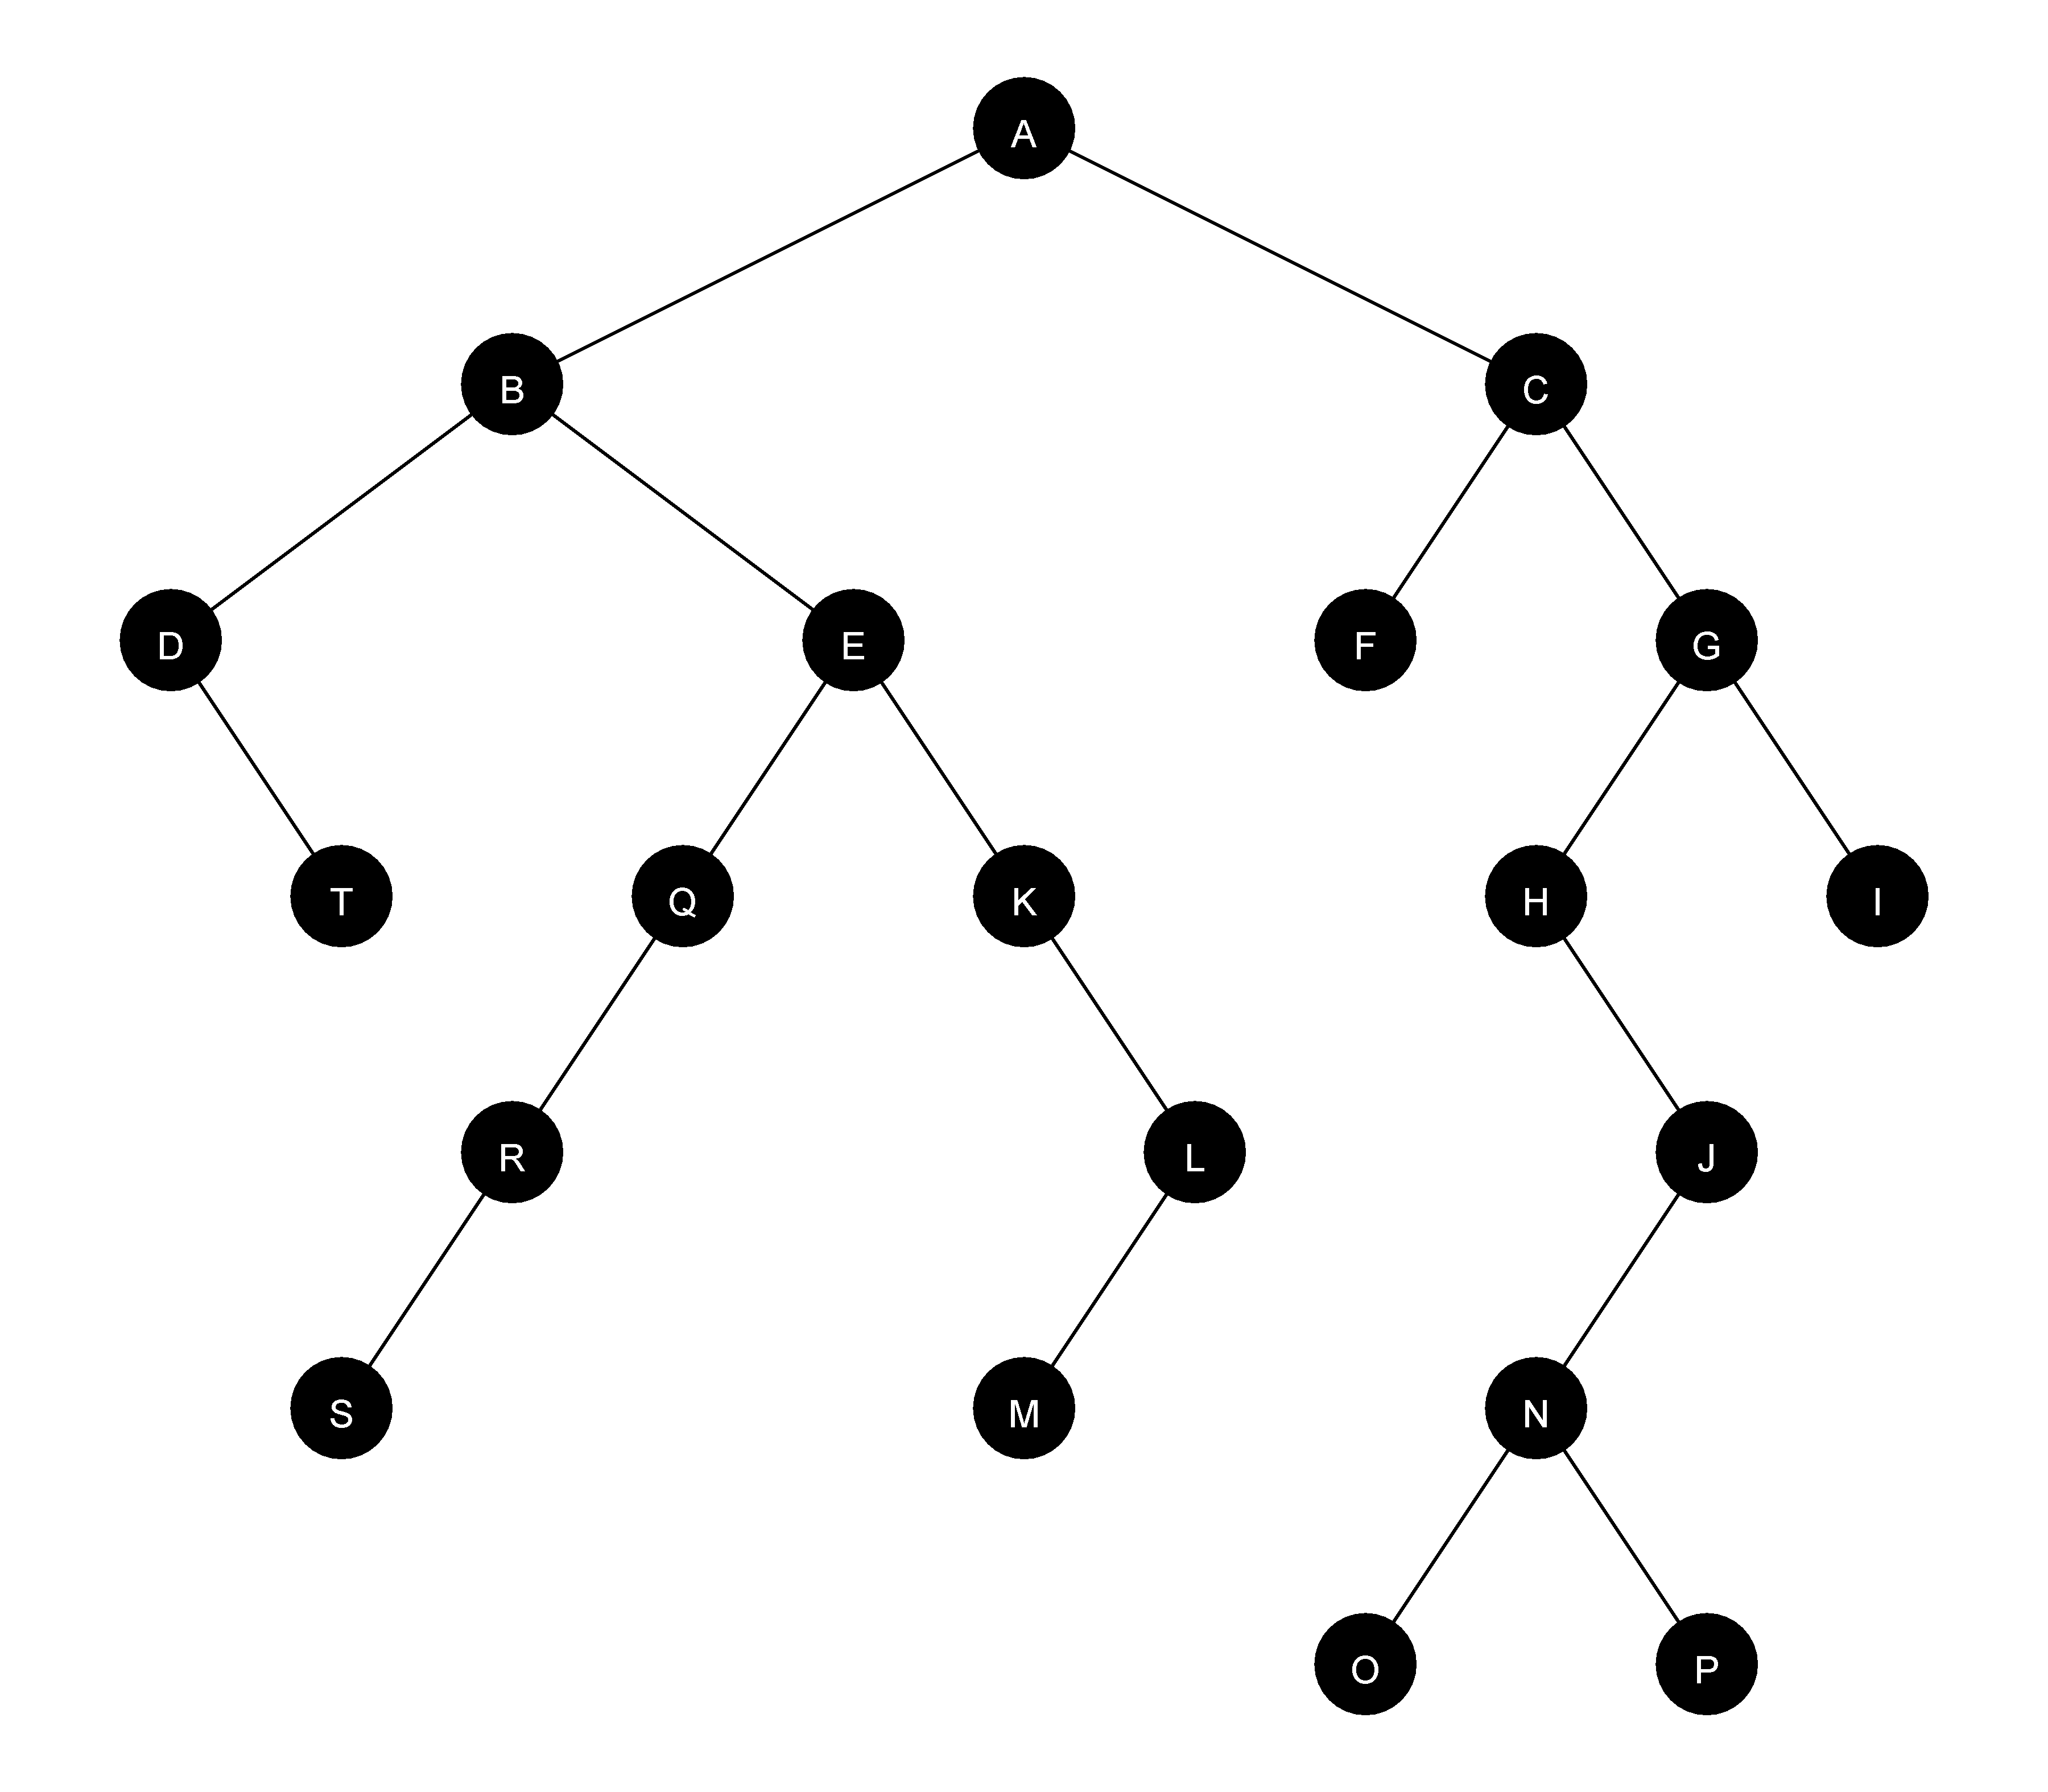
\includegraphics[scale = 0.11]{abbildungen/komplex_a3}
    \caption{Komplexer Baum gezeichnet von TR}
\end{figure}

\chapter{Anhang B}
\label{chap:anhang_b}

\lstinputlisting[caption={Knoten-Klasse}]{abbildungen/git/src/algos/Knoten.java}

\lstinputlisting[caption={Binary-Klasse}]{abbildungen/git/src/algos/BinaryKnoten.java}

\lstinputlisting[caption={WS-Naiver-Algorithmus-Klasse}]{abbildungen/git/src/algos/NaiverAlgorithmus.java}

\lstinputlisting[caption={WS-Algorithmus-Klasse}]{abbildungen/git/src/algos/VerbesserterAlgorithmus.java}

\lstinputlisting[caption={RT-Algorithmus-Klasse}]{abbildungen/git/src/algos/TilfordAlgorithmus.java}

\lstinputlisting[caption={Zusatzklasse: Trees}]{abbildungen/git/src/algos/Trees.java}

\lstinputlisting[caption={Zusatzklasse: Drawer}]{abbildungen/git/src/algos/Drawer.java}

\lstinputlisting[caption={Zusatzklasse: Mains}]{abbildungen/git/src/algos/Mains.java}